
%% bare_conf.tex
%% V1.4b
%% 2015/08/26
%% by Michael Shell
%% See:
%% http://www.michaelshell.org/
%% for current contact information.
%%
%% This is a skeleton file demonstrating the use of IEEEtran.cls
%% (requires IEEEtran.cls version 1.8b or later) with an IEEE
%% conference paper.
%%
%% Support sites:
%% http://www.michaelshell.org/tex/ieeetran/
%% http://www.ctan.org/pkg/ieeetran
%% and
%% http://www.ieee.org/

%%*************************************************************************
%% Legal Notice:
%% This code is offered as-is without any warranty either expressed or
%% implied; without even the implied warranty of MERCHANTABILITY or
%% FITNESS FOR A PARTICULAR PURPOSE! 
%% User assumes all risk.
%% In no event shall the IEEE or any contributor to this code be liable for
%% any damages or losses, including, but not limited to, incidental,
%% consequential, or any other damages, resulting from the use or misuse
%% of any information contained here.
%%
%% All comments are the opinions of their respective authors and are not
%% necessarily endorsed by the IEEE.
%%
%% This work is distributed under the LaTeX Project Public License (LPPL)
%% ( http://www.latex-project.org/ ) version 1.3, and may be freely used,
%% distributed and modified. A copy of the LPPL, version 1.3, is included
%% in the base LaTeX documentation of all distributions of LaTeX released
%% 2003/12/01 or later.
%% Retain all contribution notices and credits.
%% ** Modified files should be clearly indicated as such, including  **
%% ** renaming them and changing author support contact information. **
%%*************************************************************************


% *** Authors should verify (and, if needed, correct) their LaTeX system  ***
% *** with the testflow diagnostic prior to trusting their LaTeX platform ***
% *** with production work. The IEEE's font choices and paper sizes can   ***
% *** trigger bugs that do not appear when using other class files.       ***                          ***
% The testflow support page is at:
% http://www.michaelshell.org/tex/testflow/



\documentclass[conference]{IEEEtran}
% Some Computer Society conferences also require the compsoc mode option,
% but others use the standard conference format.
%
% If IEEEtran.cls has not been installed into the LaTeX system files,
% manually specify the path to it like:
% \documentclass[conference]{../sty/IEEEtran}

% Some very useful LaTeX packages include:
% (uncomment the ones you want to load)


% *** MISC UTILITY PACKAGES ***

\usepackage{blindtext}
\usepackage{graphicx}
\usepackage{multirow}
\usepackage{threeparttable}

%
%\usepackage{ifpdf}
% Heiko Oberdiek's ifpdf.sty is very useful if you need conditional
% compilation based on whether the output is pdf or dvi.
% usage:
% \ifpdf
%   % pdf code
% \else
%   % dvi code
% \fi
% The latest version of ifpdf.sty can be obtained from:
% http://www.ctan.org/pkg/ifpdf
% Also, note that IEEEtran.cls V1.7 and later provides a builtin
% \ifCLASSINFOpdf conditional that works the same way.
% When switching from latex to pdflatex and vice-versa, the compiler may
% have to be run twice to clear warning/error messages.






% *** CITATION PACKAGES ***
%
%\usepackage{cite}
% cite.sty was written by Donald Arseneau
% V1.6 and later of IEEEtran pre-defines the format of the cite.sty package
% \cite{} output to follow that of the IEEE. Loading the cite package will
% result in citation numbers being automatically sorted and properly
% "compressed/ranged". e.g., [1], [9], [2], [7], [5], [6] without using
% cite.sty will become [1], [2], [5]--[7], [9] using cite.sty. cite.sty's
% \cite will automatically add leading space, if needed. Use cite.sty's
% noadjust option (cite.sty V3.8 and later) if you want to turn this off
% such as if a citation ever needs to be enclosed in parenthesis.
% cite.sty is already installed on most LaTeX systems. Be sure and use
% version 5.0 (2009-03-20) and later if using hyperref.sty.
% The latest version can be obtained at:
% http://www.ctan.org/pkg/cite
% The documentation is contained in the cite.sty file itself.






% *** GRAPHICS RELATED PACKAGES ***
%
\ifCLASSINFOpdf
  % \usepackage[pdftex]{graphicx}
  % declare the path(s) where your graphic files are
  % \graphicspath{{../pdf/}{../jpeg/}}
  % and their extensions so you won't have to specify these with
  % every instance of \includegraphics
  % \DeclareGraphicsExtensions{.pdf,.jpeg,.png}
\else
  % or other class option (dvipsone, dvipdf, if not using dvips). graphicx
  % will default to the driver specified in the system graphics.cfg if no
  % driver is specified.
  % \usepackage[dvips]{graphicx}
  % declare the path(s) where your graphic files are
  % \graphicspath{{../eps/}}
  % and their extensions so you won't have to specify these with
  % every instance of \includegraphics
  % \DeclareGraphicsExtensions{.eps}
\fi
% graphicx was written by David Carlisle and Sebastian Rahtz. It is
% required if you want graphics, photos, etc. graphicx.sty is already
% installed on most LaTeX systems. The latest version and documentation
% can be obtained at: 
% http://www.ctan.org/pkg/graphicx
% Another good source of documentation is "Using Imported Graphics in
% LaTeX2e" by Keith Reckdahl which can be found at:
% http://www.ctan.org/pkg/epslatex
%
% latex, and pdflatex in dvi mode, support graphics in encapsulated
% postscript (.eps) format. pdflatex in pdf mode supports graphics
% in .pdf, .jpeg, .png and .mps (metapost) formats. Users should ensure
% that all non-photo figures use a vector format (.eps, .pdf, .mps) and
% not a bitmapped formats (.jpeg, .png). The IEEE frowns on bitmapped formats
% which can result in "jaggedy"/blurry rendering of lines and letters as
% well as large increases in file sizes.
%
% You can find documentation about the pdfTeX application at:
% http://www.tug.org/applications/pdftex





% *** MATH PACKAGES ***

\usepackage[cmex10]{amsmath}
\usepackage{amsfonts}

%
%\usepackage{amsmath}
% A popular package from the American Mathematical Society that provides
% many useful and powerful commands for dealing with mathematics.
%
% Note that the amsmath package sets \interdisplaylinepenalty to 10000
% thus preventing page breaks from occurring within multiline equations. Use:
%\interdisplaylinepenalty=2500
% after loading amsmath to restore such page breaks as IEEEtran.cls normally
% does. amsmath.sty is already installed on most LaTeX systems. The latest
% version and documentation can be obtained at:
% http://www.ctan.org/pkg/amsmath





% *** SPECIALIZED LIST PACKAGES ***
%
%\usepackage{algorithmic}
% algorithmic.sty was written by Peter Williams and Rogerio Brito.
% This package provides an algorithmic environment fo describing algorithms.
% You can use the algorithmic environment in-text or within a figure
% environment to provide for a floating algorithm. Do NOT use the algorithm
% floating environment provided by algorithm.sty (by the same authors) or
% algorithm2e.sty (by Christophe Fiorio) as the IEEE does not use dedicated
% algorithm float types and packages that provide these will not provide
% correct IEEE style captions. The latest version and documentation of
% algorithmic.sty can be obtained at:
% http://www.ctan.org/pkg/algorithms
% Also of interest may be the (relatively newer and more customizable)
% algorithmicx.sty package by Szasz Janos:
% http://www.ctan.org/pkg/algorithmicx




% *** ALIGNMENT PACKAGES ***
%
%\usepackage{array}
% Frank Mittelbach's and David Carlisle's array.sty patches and improves
% the standard LaTeX2e array and tabular environments to provide better
% appearance and additional user controls. As the default LaTeX2e table
% generation code is lacking to the point of almost being broken with
% respect to the quality of the end results, all users are strongly
% advised to use an enhanced (at the very least that provided by array.sty)
% set of table tools. array.sty is already installed on most systems. The
% latest version and documentation can be obtained at:
% http://www.ctan.org/pkg/array


% IEEEtran contains the IEEEeqnarray family of commands that can be used to
% generate multiline equations as well as matrices, tables, etc., of high
% quality.




% *** SUBFIGURE PACKAGES ***
%\ifCLASSOPTIONcompsoc
%  \usepackage[caption=false,font=normalsize,labelfont=sf,textfont=sf]{subfig}
%\else
%  \usepackage[caption=false,font=footnotesize]{subfig}
%\fi
% subfig.sty, written by Steven Douglas Cochran, is the modern replacement
% for subfigure.sty, the latter of which is no longer maintained and is
% incompatible with some LaTeX packages including fixltx2e. However,
% subfig.sty requires and automatically loads Axel Sommerfeldt's caption.sty
% which will override IEEEtran.cls' handling of captions and this will result
% in non-IEEE style figure/table captions. To prevent this problem, be sure
% and invoke subfig.sty's "caption=false" package option (available since
% subfig.sty version 1.3, 2005/06/28) as this is will preserve IEEEtran.cls
% handling of captions.
% Note that the Computer Society format requires a larger sans serif font
% than the serif footnote size font used in traditional IEEE formatting
% and thus the need to invoke different subfig.sty package options depending
% on whether compsoc mode has been enabled.
%
% The latest version and documentation of subfig.sty can be obtained at:
% http://www.ctan.org/pkg/subfig




% *** FLOAT PACKAGES ***
%
%\usepackage{fixltx2e}
% fixltx2e, the successor to the earlier fix2col.sty, was written by
% Frank Mittelbach and David Carlisle. This package corrects a few problems
% in the LaTeX2e kernel, the most notable of which is that in current
% LaTeX2e releases, the ordering of single and double column floats is not
% guaranteed to be preserved. Thus, an unpatched LaTeX2e can allow a
% single column figure to be placed prior to an earlier double column
% figure.
% Be aware that LaTeX2e kernels dated 2015 and later have fixltx2e.sty's
% corrections already built into the system in which case a warning will
% be issued if an attempt is made to load fixltx2e.sty as it is no longer
% needed.
% The latest version and documentation can be found at:
% http://www.ctan.org/pkg/fixltx2e


%\usepackage{stfloats}
% stfloats.sty was written by Sigitas Tolusis. This package gives LaTeX2e
% the ability to do double column floats at the bottom of the page as well
% as the top. (e.g., "\begin{figure*}[!b]" is not normally possible in
% LaTeX2e). It also provides a command:
%\fnbelowfloat
% to enable the placement of footnotes below bottom floats (the standard
% LaTeX2e kernel puts them above bottom floats). This is an invasive package
% which rewrites many portions of the LaTeX2e float routines. It may not work
% with other packages that modify the LaTeX2e float routines. The latest
% version and documentation can be obtained at:
% http://www.ctan.org/pkg/stfloats
% Do not use the stfloats baselinefloat ability as the IEEE does not allow
% \baselineskip to stretch. Authors submitting work to the IEEE should note
% that the IEEE rarely uses double column equations and that authors should try
% to avoid such use. Do not be tempted to use the cuted.sty or midfloat.sty
% packages (also by Sigitas Tolusis) as the IEEE does not format its papers in
% such ways.
% Do not attempt to use stfloats with fixltx2e as they are incompatible.
% Instead, use Morten Hogholm'a dblfloatfix which combines the features
% of both fixltx2e and stfloats:
%
% \usepackage{dblfloatfix}
% The latest version can be found at:
% http://www.ctan.org/pkg/dblfloatfix




% *** PDF, URL AND HYPERLINK PACKAGES ***
%
%\usepackage{url}
% url.sty was written by Donald Arseneau. It provides better support for
% handling and breaking URLs. url.sty is already installed on most LaTeX
% systems. The latest version and documentation can be obtained at:
% http://www.ctan.org/pkg/url
% Basically, \url{my_url_here}.




% *** Do not adjust lengths that control margins, column widths, etc. ***
% *** Do not use packages that alter fonts (such as pslatex).         ***
% There should be no need to do such things with IEEEtran.cls V1.6 and later.
% (Unless specifically asked to do so by the journal or conference you plan
% to submit to, of course. )


% correct bad hyphenation here
\hyphenation{op-tical net-works semi-conduc-tor}


\begin{document}
%
% paper title
% Titles are generally capitalized except for words such as a, an, and, as,
% at, but, by, for, in, nor, of, on, or, the, to and up, which are usually
% not capitalized unless they are the first or last word of the title.
% Linebreaks \\ can be used within to get better formatting as desired.
% Do not put math or special symbols in the title.
\title{Optimal Dispatch of Electrified Autonomous Mobility on Demand Vehicles during Power Outages}


% % author names and affiliations
% % use a multiple column layout for up to three different
% % affiliations
% \author{\IEEEauthorblockN{Laurel Dunn and Sangjae Bae and Max Gardner and Colin Sheppard}
% \IEEEauthorblockA{Department of Civil \& Environmental Engineering\\
% University of California, Berkeley\\
% Berkeley, CA 30332--0250\\
% Email: lndunn@lbl.gov}
% \and
% \IEEEauthorblockN{Homer Simpson}
% \IEEEauthorblockA{Twentieth Century Fox\\
% Springfield, USA\\
% Email: homer@thesimpsons.com}
% \and
% \IEEEauthorblockN{James Kirk\\ and Montgomery Scott}
% \IEEEauthorblockA{Starfleet Academy\\
% San Francisco, California 96678--2391\\
% Telephone: (800) 555--1212\\
% Fax: (888) 555--1212}}

% conference papers do not typically use \thanks and this command
% is locked out in conference mode. If really needed, such as for
% the acknowledgment of grants, issue a \IEEEoverridecommandlockouts
% after \documentclass

% for over three affiliations, or if they all won't fit within the width
% of the page, use this alternative format:
% 
\author{
\IEEEauthorblockN{Colin Sheppard\IEEEauthorrefmark{1}\IEEEauthorrefmark{2}}
\IEEEauthorblockA{colin.sheppard@berkeley.edu}
\and
\IEEEauthorblockN{Laurel N. Dunn\IEEEauthorrefmark{1}\IEEEauthorrefmark{2}}
\IEEEauthorblockA{lndunn@lbl.gov}
\and
\IEEEauthorblockN{Sangjae Bae\IEEEauthorrefmark{1}\IEEEauthorrefmark{2}}
\IEEEauthorblockA{sbae@lbl.gov}
\and
\IEEEauthorblockN{Max Gardner\IEEEauthorrefmark{1}}
\IEEEauthorblockA{magardner@berkeley.edu}
\and
\IEEEauthorblockA{\IEEEauthorrefmark{1}Dept of Civil \& Environmental Engineering\\
University of California Berkeley,
Berkeley, CA 94720}
\and
\IEEEauthorblockA{\IEEEauthorrefmark{2}Lawrence Berkeley National Laboratory\\
Berkeley, CA 94720}}




% use for special paper notices
%\IEEEspecialpapernotice{(Invited Paper)}




% make the title area
\maketitle

% As a general rule, do not put math, special symbols or citations
% in the abstract
\begin{abstract}
The era of fully autonomous, electrified taxi fleets is rapidly approaching, and with it the opportunity to innovate myriad on-demand services that extend beyond the realm of human mobility. This project envisions a future where autonomous plug-in electric vehicle (PEV) fleets can be dispatched as both a taxi service and a source of on-demand power serving customers during power outages. We develop a PDE-based scheme to manage the optimal dispatch of an autonomous fleet to serve passengers and electric power demand during outages as an additional stream of revenue. We use real world power outage and taxi data from San Francisco for our case study, modeling the optimal dispatch of several fleet sizes over the course of one day; we examine both moderate and extreme outage scenarios. In the moderate scenario, the revenue earned serving power demand is negligible compared with revenue earned serving passenger trips. In the extreme scenario, supplying power accounts for between \$1 and \$2 million, amounting to between 32\% and 40\% more revenue than is earned serving mobility only, depending on fleet size. While the overall value of providing on-demand power depends on the frequency and severity of power outages, our results show that serving power demand during large-scale outages can provide a substantial value stream, comparable to the value to be earned providing grid services.
\end{abstract}

% no keywords




% For peer review papers, you can put extra information on the cover
% page as needed:
% \ifCLASSOPTIONpeerreview
% \begin{center} \bfseries EDICS Category: 3-BBND \end{center}
% \fi
%
% For peerreview papers, this IEEEtran command inserts a page break and
% creates the second title. It will be ignored for other modes.
\IEEEpeerreviewmaketitle



\section{Introduction}
% no \IEEEPARstart
\subsection{Motivation and Background}
Fully autonomous PEVs have tremendous potential to change the future of mobility. In particular, fleets of autonomous vehicles providing on-demand mobility services will likely play a major role in transportation systems. While the impact of these changes on travel demand is uncertain, it is clear that safety, energy efficiency, and cost of travel will be substantially improved in the future. It is also clear that autonomous on-demand fleets of PEVs will require continued innovation in methods for systems optimization and control.

Autonomous PEV fleets could play an important role in providing flexibility services to the future electric grid. Another opportunity for grid-connected PEVs to add value is to supply electricity to buildings experiencing power outages when utility customers are willing to pay more for energy to avoid incurring further damages (e.g., due to business closures or food waste). The current work examines the additional revenue available to a fleet of autonomous PEVs dispatched to provide both a mobility-on-demand service and backup power during outages.

\subsection{Relevant Literature}
The current personal vehicle ownership paradigm involves gross under-utilization of vehicles, as personal vehicles sit idle for most of the day. This under-utilization makes grid-connected PEV batteries an excellent source of load flexibility, as they can charge or discharge as needed while vehicles are not in use. Numerous studies examine the capabilities \cite{lefloch_pde_2016, lefloch_pde_2015, ota_autonomous_v2g, behrouz_2014} and economics \cite{ota_autonomous_v2g} of using electric vehicles to provide grid services. A more limited body of research examines opportunities for vehicles (specifically PHEVs) to provide backup power to homes during outages \cite{shin2016}.

Current trends suggest that the future of transportation is autonomous. Once autonomous vehicles are deployed at scale, the current paradigm of personal vehicle ownership is likely to change. A commercially operated fleet of autonomous PEVs will be more heavily utilized (and thus less flexible) than privately owned vehicles are today. However, centralized control can increase the magnitude and reliability of aggregate response when price signals are adequate. 

\subsection{Focus of this Study}
We propose a PDE-based approach, described in \cite{lefloch_pde_2016}, to simulate the optimal dispatch of autonomous on-demand PEVs serving time varying, spatially distributed demand for mobility (passenger trips) and backup power. The fleet is dispatched to maximize profit earned from serving both passenger trips and power. The revenue earned for each trip serviced or kWh provided depends on the origin and destination of the trip, and the location of the power outage. We consider several fleet sizes, examining differences in vehicle dispatch, revenue earned, and unserved demand for trips/power. Key contributions of this work include the geospatial modeling of vehicle mobility, charging \& discharging, and inclusion of backup power as an ancillary revenue stream.

\section{Technical Description}
\subsection{Modeling Aggregations of Autonomous Electric Vehicles}
\begin{table}[!htbp]
% increase table row spacing, adjust to taste
\renewcommand{\arraystretch}{1.3}
% if using array.sty, it might be a good idea to tweak the value of
% \extrarowheight as needed to properly center the text within the cells
\caption{Nomenclature}
\label{tab:symbols}
\centering
\def\colmargin{6.75cm}
% Some packages, such as MDW tools, offer better commands for making tables
% than the plain LaTeX2e tabular which is used here.
\begin{tabular}{ll}
\hline
\textbf{Symbol} & \textbf{Description}\\
\hline
$x$ & PEV Battery SOE ($dx=0.2$) \\
$t$ & Time ($dt=10 min$) \\
$N_n$ & Number of nodes ($3$)\\
$N_b$ & Number of spatial bins\\
$E_{max}$ & Battery energy capacity ($10 kWh$) \\
$\eta$ & Power conversion efficiency during charging ($0.86$) \cite{veic_2013} \\
$u_i(x,t)$ & Density of charging PEVs in node $i$\\
$v_i(x,t)$ & Density of idle PEVs in node $i$\\
$w_i(x,t)$ & Density of discharging PEVs in node $i$\\
$\sigma_{I_i \rightarrow C_i}(x,t)$ & \parbox[t]{\colmargin}{ \raggedright Flow of PEVs in node $i$ from Idle to Charging} \\
$\sigma_{I_i \rightarrow D_i}(x,t)$ & \parbox[t]{\colmargin}{Flow of PEVs in node $i$ from Idle to Discharging} \\
$\sigma_{I_i \rightarrow I_j}^o(x,t)$ & \parbox[t]{\colmargin}{Flow of PEVs from Idle state of node $i$ to Idle state of node $j$ without passengers} \\
$\sigma_{I_i \rightarrow I_j}^\prime(x,t)$ & \parbox[t]{\colmargin}{ Flow of PEVs from Idle state of node $i$ to Idle state of node $j$ with passengers} \\
$q_C(x,t)$ & Instantaneous charging power \\
$q_D(x,t)$ & Instantaneous discharging power \\
$Z$ & Set of Transportation Network Nodes (I, II, IV) (see Figure \ref{fig:sf}) \\
$T$ & Time horizon of the optimization ($50 min$) \\
$\rho_{dis}(i)$ & Price of servicing load during power outages by node(\$/kWh) \\
$\rho_{mob}(i,j)$ & \parbox[t]{\colmargin}{ Price of servicing mobility demand from node $i$ to node $j$ (\$/trip/minute)} \\
\hline
\end{tabular}
\end{table}
We adopt and extend the scheme developed by \cite{lefloch_pde_2016} for tracking and controlling an aggregation of electric vehicles. The core advantage of the scheme is the recognition that in an autonomous PEV fleet, only the location of vehicles and their state of charge are critical to know at any point in time. Instead of representing individual vehicles explicitly and developing a combinatorial approach to control, we aggregate all vehicles in a node and represent the aggregate distribution of vehicle state of energy (SOE). Vehicles in any node $i$ can be in one of three states: charging, idle, or discharging, which we represent by the state variables $u_i(x,t)$, $v_i(x,t)$, and $w_i(x,t)$, respectively. The system is then characterized by the following coupled partial differential equations (see Table \ref{tab:symbols} for further nomenclature):
\begin{eqnarray*}
    \frac{\partial u_i}{\partial t}(x,t) &=& -\frac{\partial}{\partial x}\left[ q_C(x) u_i(x,t) \right] + \sigma_{I_i \rightarrow C_i}(x,t) \\
    \frac{\partial v_i}{\partial t}(x,t) &=& \sum_{j\in Z} \left[ \sigma_{I_i \leftarrow I_j}^\prime(x,t) + \sigma_{I_i \leftarrow I_j}^o(x,t) \right. \\
    & & ~~~ \left. - \sigma_{I_i \rightarrow I_j}^\prime(x,t) - \sigma_{I_i \rightarrow I_j}^o(x,t) \right] \\
    && ~~~ - \sigma_{I_i \rightarrow C_i}(x,t) - \sigma_{I_i \rightarrow D_i}(x,t) \\
    \frac{\partial w_i}{\partial t}(x,t) &=& -\frac{\partial}{\partial x}\left[ q_D(x) w_i(x,t) \right] + \sigma_{I_i \rightarrow D_i}(x,t) 
\end{eqnarray*}
Where: 
\begin{eqnarray*}
q_C(x) &=& \frac{7}{E_{max}}\eta\frac{1}{60} \\
q_D(x) &=& \frac{-7}{E_{max}}\frac{1}{60}
\end{eqnarray*}
The equations make use of an advection term (when the time derivative is linearly related to the spatial derivative) to represent how SOE changes over time for vehicles in the charging or discharging states, with SOE advecting toward 1 or 0, respectively. The model is spatially disaggregated, so the three PDEs are repeated for every node in the system and indexed by $i$.

Flow terms $\sigma_{I_i \rightarrow C_i}(x,t)$ and $\sigma_{I_i \rightarrow D_i}(x,t)$ capture the transport of vehicles between the SOE curves for each state at a particular node. Additional flow terms capture transport between the Idle curves of different nodes. For a given node $i$ and any other node $j$, four separate terms represent trips with/without passengers ($\sigma^\prime$ and $\sigma^o$ respectively) and departing from/arriving at the node ($\sigma_{I_i \rightarrow I_j}$ and $\sigma_{I_j \leftarrow I_i}$ respectively). Collectively, all terms denoted by $\sigma$ are decision variables, where departures and arrivals are coupled via the constraints (as discussed below).

The inter-nodal flow terms are constrained such that departures from a node $i$ to node $j$ are equivalent to the arrivals of vehicles from $i$ to $j$ at a future time and with a lower SOE, corresponding to the travel time and energy requirements of that trip, as specified in Table \ref{tab:flow_constraints}. The distinction between trips with and without passengers becomes critical in the context of the economic optimization that places monetary value on transporting people but not on moving empty vehicles. Though we do account for the energy costs associated with moving empty vehicles, we do not consider the costs of any congestion these vehicles may cause.

\subsection{Optimization Formulation}
\subsubsection{Objective}
The objective of the optimization is to maximize the operational profit of dispatching the fleet of autonomous on-demand PEVs:
\begin{eqnarray*}
  \max_{\substack{\sigma_{I_i \rightarrow C_i} \\
    \sigma_{I_i \rightarrow D_i} \\ 
    \sigma_{I_i \rightarrow I_j}}}
    K &=& \sum_{i\in Z} \int_{t=0}^{T} \left[ \frac{\rho_{dis}(i)}{60} Q_{dis,i}(t) + \right. \\ 
      && \left. \sum_{j\in Z}\rho_{mob}(i,j)Q_{mob,i,j}(t)  - \frac{C}{60}Q_{ch,i}(t) \right]dt\\
    Q_{dis,i}(t) & = & \int_{0}^{1} 7 w_i(x,t) dx \\
    Q_{ch,i}(t) & = & \int_{0}^{1} 7 u_i(x,t) dx \\
    Q_{mob,i,j}(t) & = & \int_{0}^{1}\left( \sigma_{I_i \rightarrow I_j}^\prime(x,t) \right)dx
\end{eqnarray*}
Where $\rho_{mob}(i,j)$, $\rho_{dis}(i)$, and $C$ are the fares charged to passengers, the price charged to serve load during outages, and the cost to purchase electricity from the grid, respectively. The constant 60 converts kWh to kW-minutes, and the constant 7 is the charging and discharging rate of each vehicle consistent with current charging/discharging rates of Level 2 chargers.

\subsubsection{Constraints}
The equations of state are discretized using a first-order upwind scheme for numerically solving hyperbolic PDEs. They appear in the formulation as a set of equality constraints. Additional constraints limit the flow of vehicles between nodes to within realistic bounds, and ensure the overall conservation of vehicles in the system.

Firstly, we constrain the size of the flows between states $u$, $v$, and $w$ to be no greater than the number of vehicles in those states:
\begin{eqnarray*}
    -\sigma_{I_i \rightarrow C_i}(x,t) & \le & u_i(x,t) / \Delta t \\
  \left\{ \sigma_{I_i \rightarrow C_i}(x,t) + \sigma_{I_i \rightarrow D_i}(x,t) \right. && \\
  + \sigma_{I_i \rightarrow I_j}^\prime(x,t) + \sigma_{I_i \rightarrow I_j}^o(x,t) && \\
  \left. - \sigma_{I_i \leftarrow I_j}^\prime(x,t) - \sigma_{I_i \leftarrow I_j}^o(x,t) \right\} & \le & v_i(x,t) / \Delta t \\
    -\sigma_{I_i \rightarrow D_i}(x,t) & \le & w_i(x,t) / \Delta t
\end{eqnarray*}
We also require that as charging vehicles reach an SOE of 1 or as discharging vehicles reach an SOE of 0, they immediately flow to the Idle state.
\begin{eqnarray*}
    -\sigma_{I_i \rightarrow C_i}(1,t) & = & u_i(1,t) / \Delta t \\
    -\sigma_{I_i \rightarrow D_i}(0,t) & = & w_i(0,t) / \Delta t
\end{eqnarray*}
Next, we require that trips be conserved between origin-destination pairs, where arrivals are shifted to a later time step and a lower SOE, based on the time ($\Delta t$) and energy ($\Delta x$) requirements of the trip.
\begin{eqnarray*}
    \sigma_{I_i \rightarrow I_j}^\prime(x,t) & = & \sigma_{I_j \leftarrow I_i}^\prime(x - \Delta x_{i,j},t + \Delta t_{i,j}) \\
     \sigma_{I_i \rightarrow I_j}^o(x,t) & = & \sigma_{I_j \leftarrow I_i}^o(x - \Delta x_{i,j},t + \Delta t_{i,j})
\end{eqnarray*}
\begin{equation*}
\{(i,j) \in Z \times Z\} 
\end{equation*}
The values of $\Delta x$ and $\Delta t$ for each node (I, II and IV shown in Figure \ref{fig:sf}) are derived from historic taxi mobility and fare datasets such as \cite{mobility2009} and \cite{fares2017}, respectively. We assume a decline in personal vehicle ownership accompanies deployment of autonomous vehicles. We account for increasing reliance on mobility-on-demand services by scaling travel demand by a factor of 10 relative to 2012. We took the average trip durations and trip distances for trips from each node $i$ to each node $j$, scaling the average distance by 5.05 km/kWh to derive $\Delta x_{i,j}$ and taking the average time as $\Delta t_{i,j}$. The derived values are shown in Table \ref{tab:flow_constraints}.
\begin{table}[!htbp]
    % increase table row spacing, adjust to taste
    \renewcommand{\arraystretch}{1}
    % if using array.sty, it might be a good idea to tweak the value of
    % \extrarowheight as needed to properly center the text within the cells
    \caption{Flow Constraints}
    \label{tab:flow_constraints}
    \centering
    \def\colmargin{6.75cm}
    % Some packages, such as MDW tools, offer better commands for making tables
    % than the plain LaTeX2e tabular which is used here.
    \begin{tabular}{lll}
    \hline
    \textbf{Node Flows ($i$ $\rightarrow$ $j$)} & \textbf{Derived} $\Delta x$ (kWh) & \textbf{Derived} $\Delta t$ (s) \\
    \hline
    I$\rightarrow$I & 0.42  & 476  \\
    I$\rightarrow$II & 0.82  & 792  \\
    I$\rightarrow$IV & 0.93  & 1000  \\
    II$\rightarrow$I & 0.84  & 760  \\
    II$\rightarrow$II & 0.38  & 489  \\
    II$\rightarrow$IV & 0.77  & 698  \\
    IV$\rightarrow$I & 0.93  & 956  \\
    IV$\rightarrow$II & 0.77  & 725  \\
    IV$\rightarrow$IV & 0.37  & 403  \\
    \hline
    \end{tabular}
\end{table}
Vehicle dispatch is constrained such that the number of vehicles servicing passenger trips or power demand cannot exceed mobility and power demand at that time step.
\begin{eqnarray*}
   Q_{dis,i}(t) & \le & D_{dis,i}(t) \\
   Q_{mob,i,j}(t) & \le & D_{mob,i,j}(t) \\
\end{eqnarray*}
The demands $D_{dis,i}$ and $D_{mob,i,j}$ are exogenously defined; derivation of $D_{dis,i}$ is described below. The choice of inequality constraints when constraining $Q_{dis,i}$ and $Q_{mob,i,j}$ serves three purposes: 1) it allows the solution of the optimization to prioritize between serving the two types of demand; 2) it enables simulations where the fleet of vehicles is not sized to meet the peak demand in the system; and 3) it allows the system to be used in an application where power outages occur spontanteously and without foresight.

Finally, we require that the vehicle batteries have sufficient energy to make trips:
\begin{eqnarray*}
    \sigma_{I_i \rightarrow I_j}^\prime(x,t) & = & 0, ~~~ x < \Delta x_{i,j} \\
    \sigma_{I_i \rightarrow I_j}^o(x,t) & = & 0, ~~~ x < \Delta x_{i,j}
\end{eqnarray*}

Both the objective function and constraints are linear, making this a linear program. We have implemented the problem in R and use lp\_solve (an implementation of the simplex method) to find the optimal solution at each time step.

\subsection{Application}
\subsubsection{Spatial Discretization}
We divided the City of San Francisco, CA into a simplified 4-zone, equal-area network illustrated in Figure \ref{fig:sf}. As described above, we construct a mobility scenario to characterize demand for passenger trips to/from/within each node, travel time beteen nodes, and taxi fares. Below we describe how power outages are characterized from real world data. We observe very little demand for mobility and few outages in Node III. Thus due to additional computational complexity of modeling a four node system, we exclude Node III from our analysis.
\begin{figure}[!htbp]
  \begin{center}
  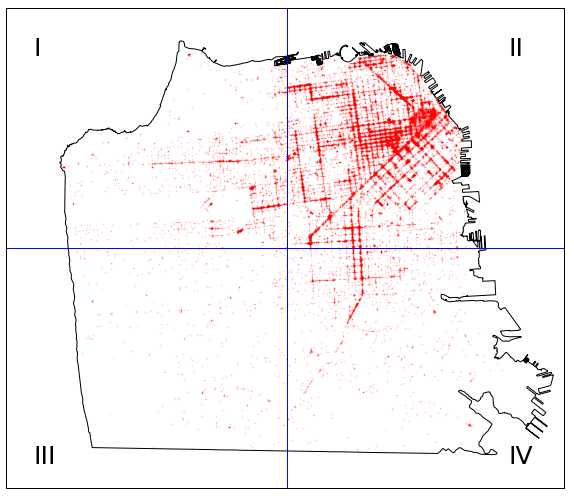
\includegraphics[width=0.6\linewidth]{plots/grid1-cropped.png}
  \end{center}
  \vspace{-5pt}
  \caption{We divide San Francisco into 4 equal-area nodes. Origin and destination of taxi trips are shown as red dots. Node III is excluded from the simulation due to limited demand.}
  \label{fig:sf}
\end{figure}
\subsubsection{Demand for Backup Power}
We estimate the magnitude and location of power outages using historic outage data collected from the Pacific Gas \& Electric Company website. The data collected include the number and spatial distribution of power outages in the region over time; we aggregate outages spatially by node. We estimate the magnitude of unserved load based on the number of customers affected, the expected number of customers by customer type (i.e., residential, commercial, industrial), and average power demand by customer type (as reported in EIA form 861). In the current implementation, we assume demand to be the same accross all customers of a particular type and constant throughout the day. We use local population and economic census data to estimate the distribution of customers by type in each node.

We examine two days of outage data, including one extreme outage scenario (December 31, 2014) and one moderate outage scenario (September 29, 2014). Figure \ref{fig:power_demand} shows the estimated power demand at each node for both scenarios. We highlight that demand in the Extreme outage scenario exceeds demand in the Moderate outage scenario by two orders of magnitude.
\begin{figure}[!htbp]
  \begin{center}
  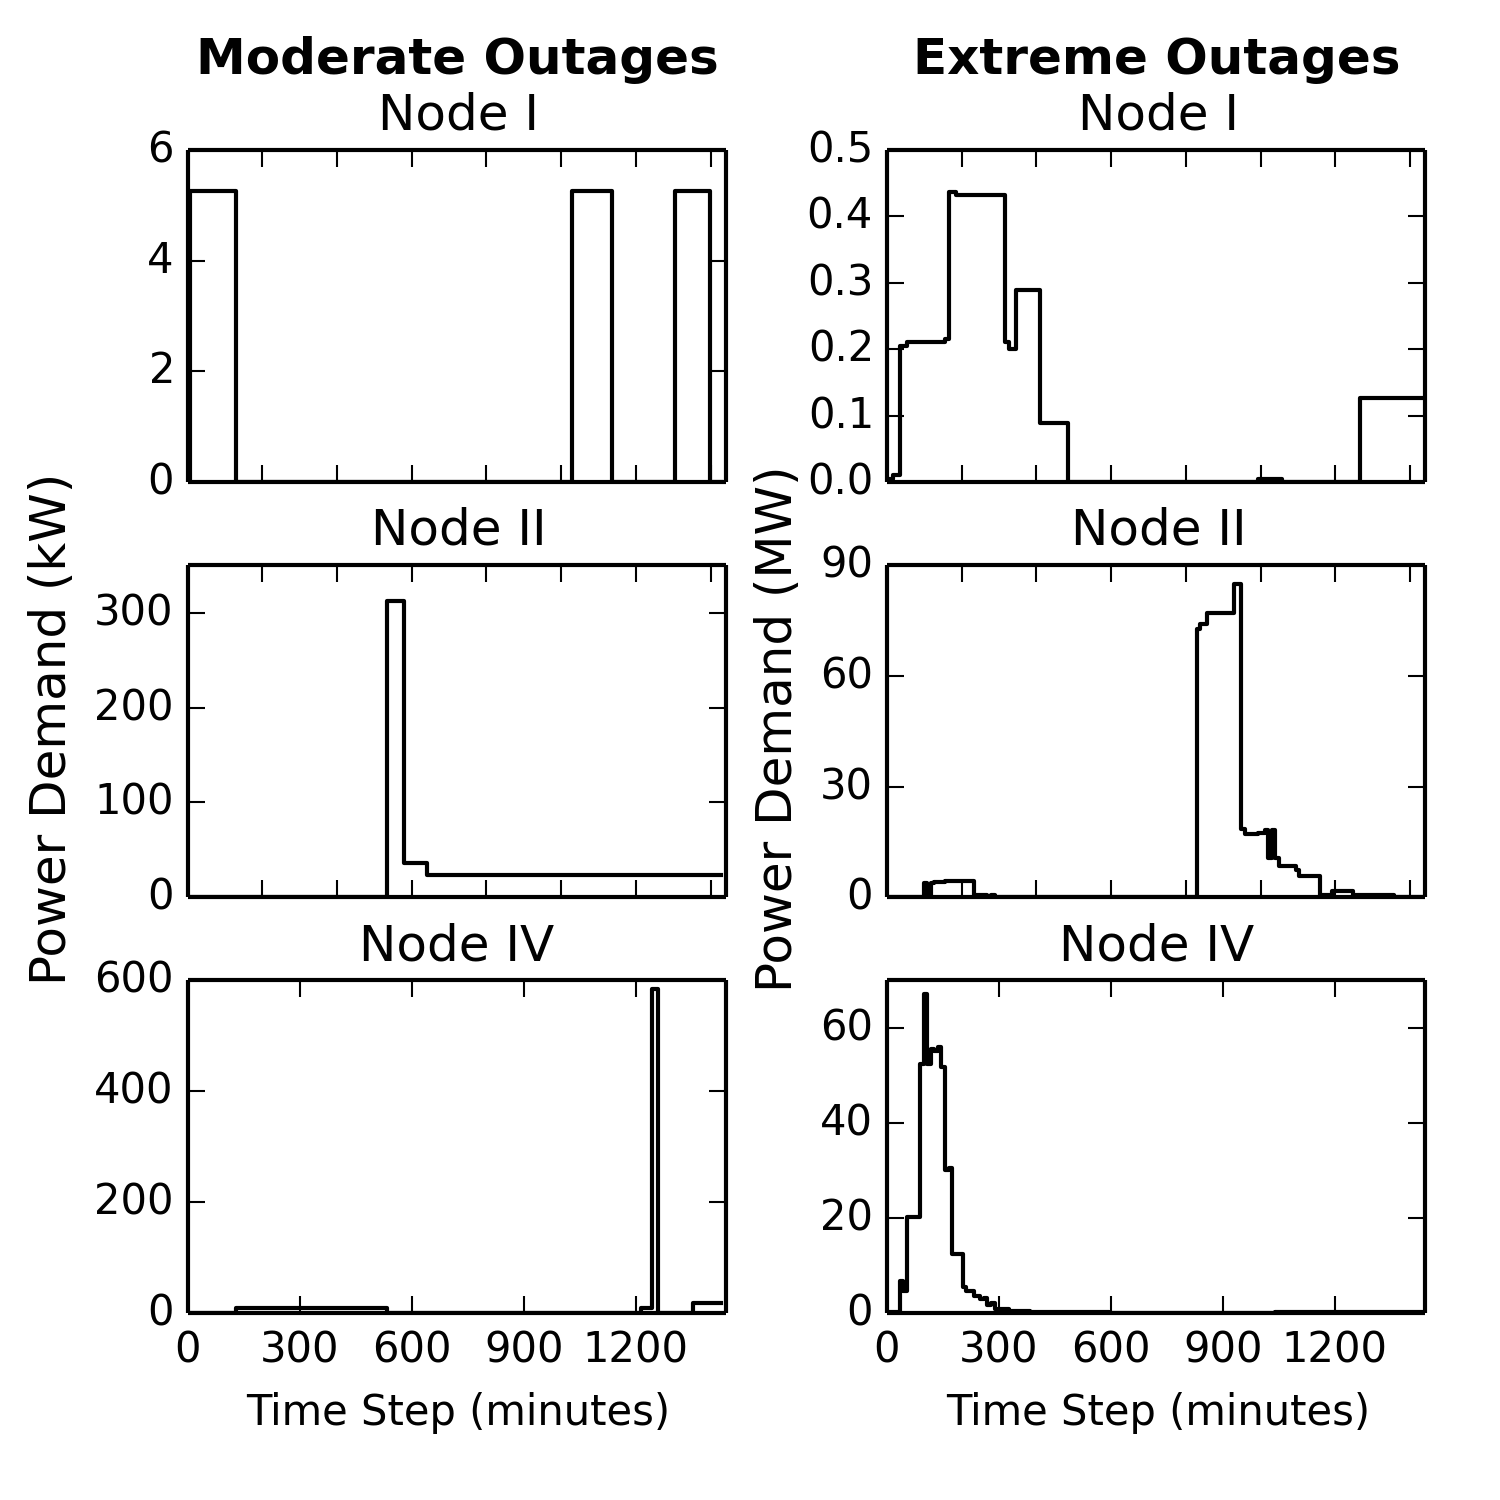
\includegraphics[width=0.8\linewidth]{plots/power_demand.png}
  \end{center}
  \vspace{-5pt}
  \caption{Power demand at each node (I, II, IV) in the Moderate (left) and Extreme (right) outage scenarios, reprsented by September 29, 2014 and December 31, 2014, respectively. For readability, demand is reported in kWh in the Moderate scenario, and in MWh in the Extreme scenario.}
  \label{fig:power_demand}
\end{figure}
Finally, we estimate the value of providing on-demand backup power by computing the cost of damages incurred due to outages in each node for both outage scenarios. We use the Interruption Cost Estimate (ICE) Calculator to do so \cite{ice_calculator_2015}. Table \ref{tab:outage_costs} gives the estimated value of backup power in each node for the two outage scenarios in \$/kWh and \$/$\Delta t$ (where $\Delta t$ is 10 minutes). Although power demand is much higher in the Extreme outages scenario, the cost per kWh is greater in the Moderate outages scenario.
\begin{table}[!htbp]
    % increase table row spacing, adjust to taste
    \renewcommand{\arraystretch}{1}
    % if using array.sty, it might be a good idea to tweak the value of
    % \extrarowheight as needed to properly center the text within the cells
    \caption{Cost of power outages in each node for Extreme and Moderate outage scenarios per kWh delivered, and per time step (10 minutes).}
    \label{tab:outage_costs}
    \centering
    \def\colmargin{6.75cm}
    % Some packages, such as MDW tools, offer better commands for making tables
    % than the plain LaTeX2e tabular which is used here.
    \begin{tabular}{lllll}
    \hline
    \multirow{2}{*}{\textbf{Node ($i$)}} & \multicolumn{2}{c}{\textbf{Extreme}} & \multicolumn{2}{c}{\textbf{Moderate}} \\
     & (\$/kWh) & (\$/$\Delta t$) & (\$/kWh) & (\$/$\Delta t$) \\
    \hline
    I  & 20 & 23 & 14 & 16 \\
    II & 9  & 11 & 32 & 37 \\
    IV & 15 & 18 & 46 & 54 \\
    \hline
    \end{tabular}
\end{table}
For comparison, Table \ref{tab:trip_costs} lists the fares associated with passenger trips to and from each node in terms of dollars per unit energy consumed (\$/kWh) and dollars per unit time (\$/$\Delta t$). We highlight that the value earned per kWh serving passenger trips is remarkably similar to the value earned per kWh of power demand served.
\begin{table}[!htbp]
    % increase table row spacing, adjust to taste
    \renewcommand{\arraystretch}{1}
    % if using array.sty, it might be a good idea to tweak the value of
    % \extrarowheight as needed to properly center the text within the cells
    \caption{Cost of passenger trips per unit energy and per unit time for each origin-destination pair.}
    \label{tab:trip_costs}
    \centering
    \def\colmargin{6.75cm}
    % Some packages, such as MDW tools, offer better commands for making tables
    % than the plain LaTeX2e tabular which is used here.
    \begin{tabular}{llll}
    \hline
    \multirow{2}{*}{\textbf{Origin}} & \multirow{2}{*}{\textbf{Destination}} & \multicolumn{2}{c}{\textbf{Cost}} \\
     &  & \$/kWh & \$/$\Delta t$ \\
    \hline
    I  & I  & 25 & 11 \\
    I  & II & 19 & 8 \\
    I  & IV & 20 & 9 \\
    II & I  & 18 & 8 \\
    II & II & 26 & 10 \\
    II & IV & 19 & 7 \\
    IV & I  & 20 & 9 \\
    IV & II & 19 & 7 \\
    IV & IV & 24 & 9 \\
    \hline
    \end{tabular}
\end{table}
\section{Results}
We present simulation results for the two outage scenarios with various fleet sizes, including 7,500, 10,000 and 15,000 vehicles for the Moderate outage scenario, and 7,500, 15,000 and 40,000 vehicles for the Extreme outage scenario. The following sections detail the results. We highlight the revenue earned in different scenarios, and differences in dispatch among different fleet sizes.

\subsection{Revenue}
Figure \ref{fig:revenue_bar} presents the revenue earned in each scenario by the entire fleet and per vehicle. Contributors to overall revenue include: the cost to charge (G2V), revenue earned serving trips (Trips), and revenue earned serving power demand (V2B). The total revenue earned (Total) in each scenario and maximum possible revenue (Max) are also shown. The maximum possible revenue includes servicing all passenger trips and all power demand, with no charing costs.
\begin{figure}[!htbp]
  \begin{center}
  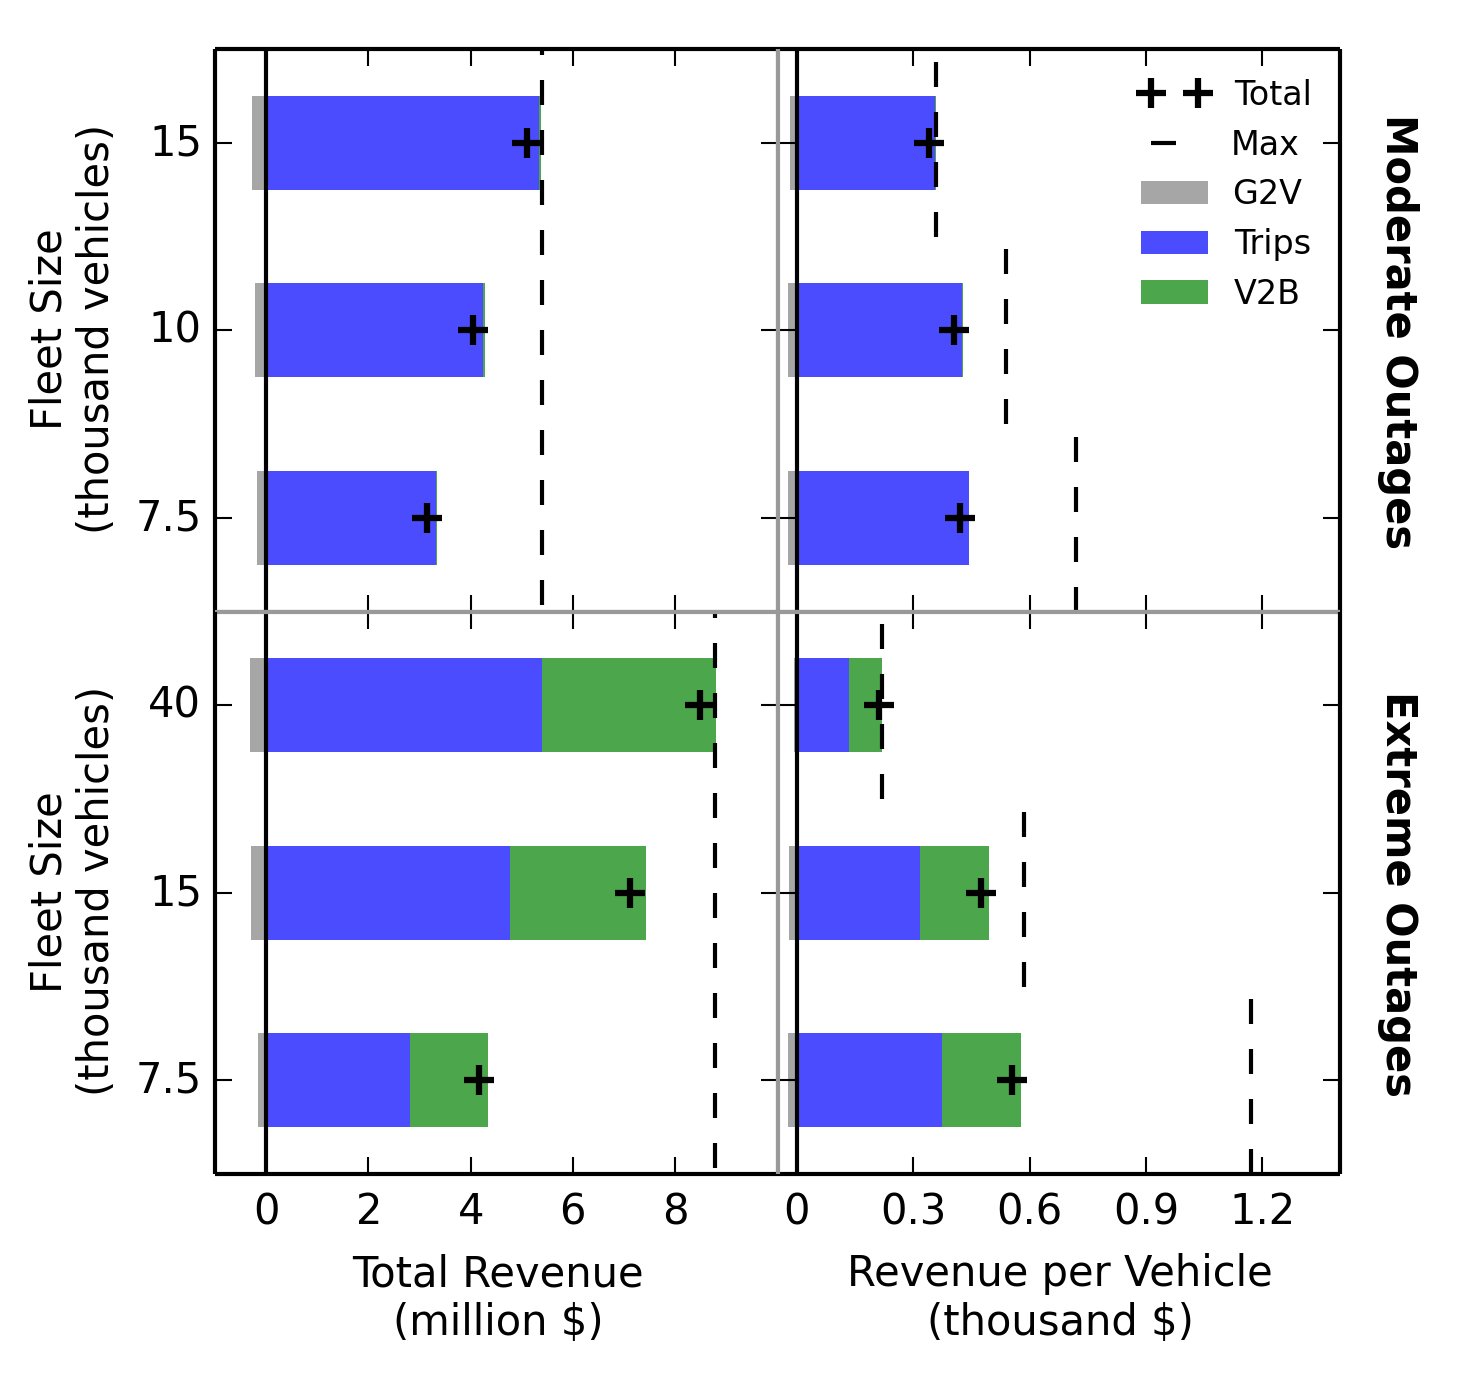
\includegraphics[width=0.8\linewidth]{plots/full_revenue_barchart.png}
  \end{center}
  \vspace{-5pt}
  \caption{Revenue earned by entire fleet (left) and per vehicle (right) in the Moderate (top) and Extreme (bottom) outage scenarios. Revenue components include: cost to charge (G2V), revenue earned serving passenger trips (Trips), and revenue earned serving power demand (V2B). The total revenue (Total) and maximum possible revenue (Max) are also shown.}
  \label{fig:revenue_bar}
\end{figure}
Charging costs are almost negligible compared with the revenue earned because the cost of charging (0.25 \$/kWh) is small compared with the revenue earned serving power and mobility demand (see Tables \ref{tab:outage_costs} and \ref{tab:trip_costs}).

\subsection{Fleet Size and Vehicle Dispatch}
Next we consider the benefits and drawbacks of different fleet sizes. Nearly all demand for mobility and power can be served with a 40,000 vehicle fleet in the Extreme scenario, and a 15,000 vehicle fleet in the Moderate scneario. Figures \ref{fig:time_extreme_40k} and \ref{fig:time_extreme_7500} show the number of vehicles in each state in the Extreme outages scenario with 40,000 and 7,500 vehicles. States include: discharging, idle, charging, and in transit both with and without passengers. 
\begin{figure}[!htbp]
  \begin{center}
  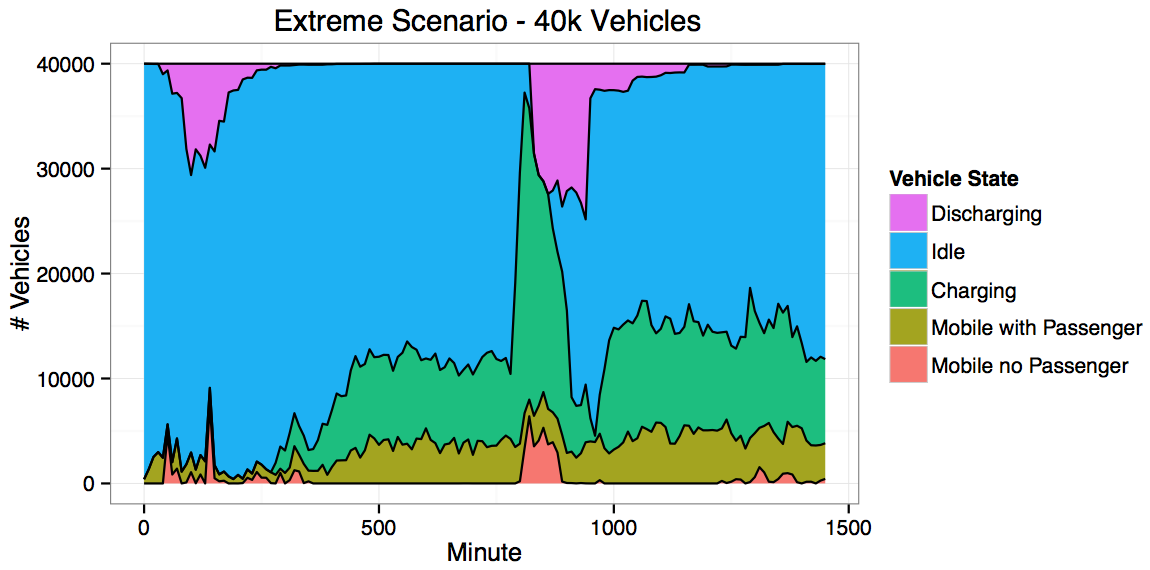
\includegraphics[width=\linewidth]{plots/states-area-40k-reverse.png}
  \end{center}
  \vspace{-5pt}
  \caption{Number of vehicles in each state at each time step in the Extreme outages scenario with a 40,000 vehicle fleet. States include: in transit with and without passengers, charging, discharging, and idle.}
  \label{fig:time_extreme_40k}
\end{figure}
\begin{figure}[!htbp]
  \begin{center}
  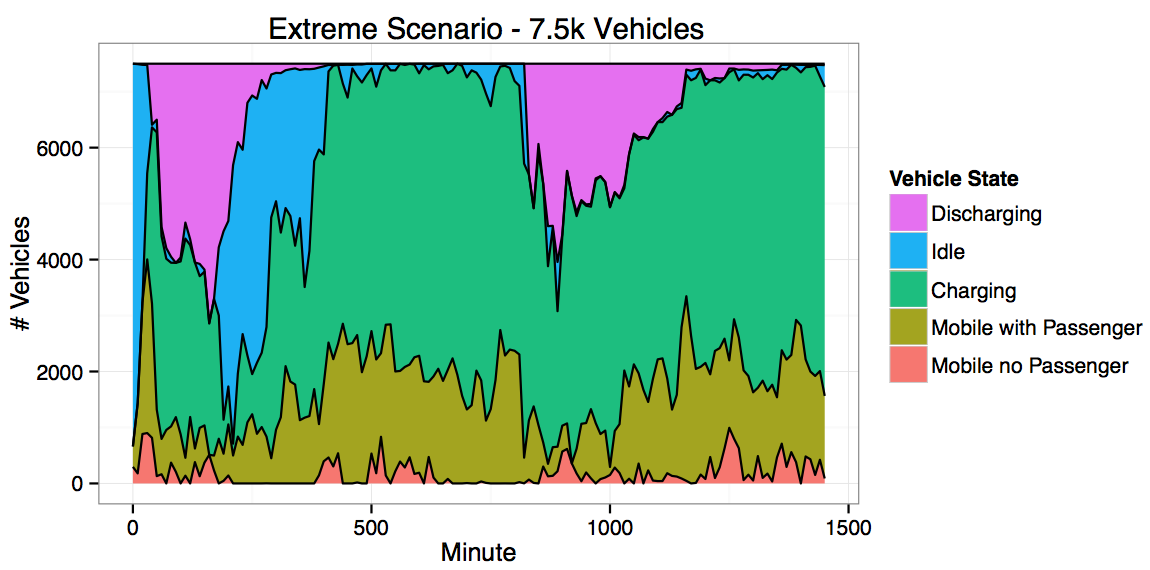
\includegraphics[width=\linewidth]{plots/states-area-7500-reverse.png}
  \end{center}
  \vspace{-5pt}
  \caption{Number of vehicles in each state at each time step in the Extreme outages scenario with a 7,500 vehicle fleet. States include: in transit with and without passengers, charging, discharging, and idle.}
  \label{fig:time_extreme_7500}
\end{figure}
Figure \ref{fig:time_extreme_40k} reveals that a 40,000 vehicle fleet spends most of the simulation in the idle state; the fleet is only fully utilized between 800 and 900 seconds when power demand peaks. Low revenue per vehicle in Figure \ref{fig:revenue_bar} provides further evidence that the 40,000 vehicle fleet is under-utilized. On the other hand, the 7,500 vehicle fleet in Figure \ref{fig:time_extreme_7500} earns less revenue overall, but spends very little time in the idle state. In fact, the vehicles spend more time charging than in any other state; faster charging infrastructure would increase fleet utilization. Future work will evaluate fast-charging infrastructure as an alternative to increasing the fleet size.
\section{Discussion}
To determine whether on-demand backup power provides a substantial value stream for the fleet, we consider the relative frequency of Extreme and Moderate outage days and the marginal revenue earned by serving power demand in addition to passenger trips. To do so, we compute the marginal annual revenue earned serving both power and mobility demand compared with serving mobility only. We examine several scenarios for the number of Extreme verses Moderate outage days in a year. We treat the Moderate outages scenario as a mobility-only scenario, as the revenue earned serving power demand in that scenario is negligible. The results are summarized in Table \ref{tab:annual_scenarios}.

\begin{threeparttable}
    % increase table row spacing, adjust to taste
    \renewcommand{\arraystretch}{1}
    % if using array.sty, it might be a good idea to tweak the value of
    % \extrarowheight as needed to properly center the text within the cells
    \caption{Increase in annual revenue from serving power demand in addition to mobility for 7,500 and 15,000 vehicle fleets with a range of scenarios regarding the number of Extreme outage days in the year.}
    \label{tab:annual_scenarios}
    \centering
    \def\colmargin{6.75cm}
    % Some packages, such as MDW tools, offer better commands for making tables
    % than the plain LaTeX2e tabular which is used here.
    \footnotesize{
    \begin{tabular}{p{1cm}p{1cm}p{1cm}p{1cm}p{1cm}}
    \hline
    \multirow{2}{1cm}{\textbf{Extreme Days}} & \multicolumn{2}{c}{\textbf{New Revenue} (\$/year/vehicle)} & \multicolumn{2}{c}{\textbf{Percent Increase} (\%)} \\
    &7,500 & 15,000 & 7,500 & 15,000 \\
    \hline
    10 & 1400 & 2000 & 0.9 & 1.6 \\
    12 & 1700 & 2300 & 1.0 & 1.8 \\
    14 & 2000 & 2600 & 1.2 & 2.0 \\
    16\tnote{\textasteriskcentered} & 2200 & 2800 & 1.4 & 2.2 \\
    18 & 2500 & 3100 & 1.5 & 2.4 \\
    20 & 2800 & 3400 & 1.7 & 2.6 \\
    \hline
    \end{tabular}
      \begin{tablenotes}
        \footnotesize
        \item[\textasteriskcentered] Actual number of days with major power outages in the Pacific Gas and Electric Company service territory in 2014 \cite{pge_reliability_2014}.
      \end{tablenotes}}
\end{threeparttable}

We calculate the marginal revenue earned serving power demand by taking the difference between each year and the annualized mobility-only scenario. Our results suggest that fleet operators can earn \$1,400-\$3,400 (or $\sim$1-3\%) additional revenue per vehicle per year serving power demand during outages, depending on fleet size and the number of major power outages.

These results are sensitive to numerous assumptions in our analysis, including but not limited to: outage cost, outage frequency/duration, outage size/scope, power demand, vehicle battery size, battery discharge rate, optimization window, and foresight into demand for power and passenger trips.

\section{Summary}
We demonstrate a method for simulating the energy and geospatial distribution of a fleet of autonomous PEVs in San Francisco dispatched to serve mobility and electricity demand during power outages. We use a PDE-based approach to model the aggregate state of energy of the fleet as vehicles charge, discharge, and travel throughout the system. We optimize vehicle dispatch over a 50 minute planning horizon, assuming perfect foresight into both mobility and power demand within that time frame. We consider two outage scenarios, including both Moderate and Extreme outages based on real outage data for San Francisco. Finally, we compute the revenue earned in each scenario with various fleet sizes, ranging from 7,500 to 40,000 vehicles. We find that serving power demand increases fleet revenue by \$1,400-\$3,400 per vehicle, or 30-40\%, in the Extreme outages scenario. Given that power outages are rare, these results translate to $\sim$1-3\% more revenue per year, depending on the number of major power outages in a year.

% use section* for acknowledgment
\section*{Acknowledgments}
The authors would like to thank Scott Moura and Caroline le Floch at UC Berkeley for advising this work. We also thank Michael Sohn and Joseph Eto at Lawrence Berkeley National Laboratory for granting us access to the outage dataset.

% trigger a \newpage just before the given reference
% number - used to balance the columns on the last page
% adjust value as needed - may need to be readjusted if
% the document is modified later
%\IEEEtriggeratref{8}
% The "triggered" command can be changed if desired:
%\IEEEtriggercmd{\enlargethispage{-5in}}

% references section

% can use a bibliography generated by BibTeX as a .bbl file
% BibTeX documentation can be easily obtained at:
% http://mirror.ctan.org/biblio/bibtex/contrib/doc/
% The IEEEtran BibTeX style support page is at:
% http://www.michaelshell.org/tex/ieeetran/bibtex/
% \bibliographystyle{IEEEtran}
% argument is your BibTeX string definitions and bibliography database(s)
% \bibliography{refs}
%
% <OR> manually copy in the resultant .bbl file
% set second argument of \begin to the number of references
% (used to reserve space for the reference number labels box)
\begin{thebibliography}{10}

\bibitem{lefloch_pde_2016}
C.~Le~Floch, E.~Kara, and S.~Moura, ``{PDE} modeling and control of electric
  vehicle fleets for ancillary services: A discrete charging case,'' \emph{IEEE
  PES Transactions on Smart Grid}, 2016.

\bibitem{lefloch_pde_2015}
C.~Le~Floch, F.~di~Meglio, and S.~Moura, ``Optimal charging of vehicle-to-grid
  fleets via {PDE} aggregation techniques,'' in \emph{American Control
  Conference}, 2015.

\bibitem{ota_autonomous_v2g}
Y.~Ota, H.~Taniguchi, T.~Nakajima, K.~M. Liyanage, J.~Baba, and A.~Yokoyama,
  ``Autonomous distributed {V2G} ({Vehicle-to-Grid}) satisfying scheduled
  charging,'' \emph{IEEE Transactions on Smart Grid}, vol.~3, no.~1, 2012.

\bibitem{behrouz_2014}
B.~Ebrahimi and J.~Mohammadpour, ``Aggregate modeling and control of plug-in
  electric vehicles for renewable power tracking,'' \emph{American Control
  Conference}, 2014.

\bibitem{shin2016}
H.~Shin and R.~Baldick, ``Plug-in electric vechile to home ({V2H}) operation
  under a grid outage,'' \emph{IEEE Transactions on Smart Grid}, 2016.

\bibitem{veic_2013}
E.~Forward, K.~Glitman, and D.~Roberts, ``An assessment of {Level} 1 and
  {Level} 2 electric vehicle charging efficiency,'' Vermont Energy Investment
  Corporation, Tech. Rep., March 2013.

\bibitem{mobility2009}
M.~Piorkowski, N.~Sarafijanovic-Djukic, and M.~Grossglauser, ``{CRAWDAD}
  dataset epfl/mobility (v. 2009-02-24),'' Downloaded from
  \url{http://crawdad.org/epfl/mobility/20090224}, feb 2009.

\bibitem{fares2017}
\BIBentryALTinterwordspacing
``San {F}rancisco taxi fare finder.'' [Online]. Available:
  \url{https://www.taxifarefinder.com/main.php?city=SF}
\BIBentrySTDinterwordspacing

\bibitem{ice_calculator_2015}
M.~J. Sullivan, J.~Schellenberg, and M.~Blundell, ``Updated value of service
  reliability estimates for electric utility customers in the {United}
  {States},'' Nexant, Inc., LBNL Report LBNL-6941E, 2015.

\bibitem{pge_reliability_2014}
{Pacific Gas and Electric Company}, ``2014 {Annual} {Electric} {Distribution}
  {Reliability} {Report},'' February 2015.


\end{thebibliography}




% that's all folks
\end{document}


